\section{Aufbau}
\label{sec:Aufbau}

\noindent Die \autoref{fig:schaltung} zeigt die schematische Darstellung des Versuchsaufbaus. 

\begin{figure}[h]
    \centering
    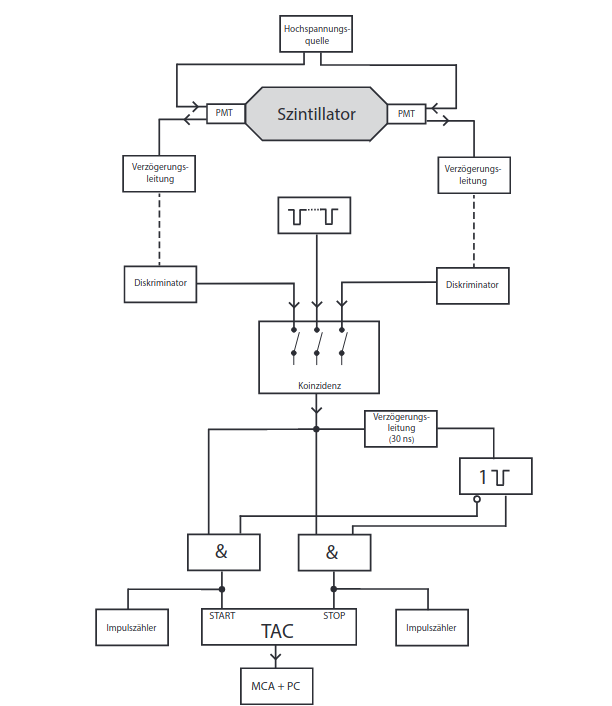
\includegraphics[width=0.8\textwidth]{bilder/blockschaltbild.png}
    \caption{Das Blockschaltbild der im Versuch benutzten Schaltung \cite{anleitung}.}
    \label{fig:schaltung}
\end{figure}

\noindent Die einfallenden Myonen werden mithilfe eines organischen Szintillationsdetektors detektiert, der Tank hat eine Größe von etwa $V = \SI{50}{\litre}$. 
In dem organischen Stoff werden die Moleküle durch das einfallende Myon oder das beim Zerfall entstehende Elektron angeregt, 
bei der Rückkehr in den Grundzustand werden Photonen mit einer Wellenlänge von etwa $\lambda \approx \SI{400}{\nano\metre}$ \cite{kalonoski} emittiert. Es entsteht 
auch Licht durch das beim Myonzerfall entstehende Elektron. Die Lichtbitze werden über Lichtleiter an Photovervielfacher (PMT) weitergegeben. In einem PMT werden die Photonen auf eine 
Photokathode gelenkt, dort werden nach dem Photoeffekt Elektronen ausgelöst. Diese werden über die anliegende Hochspannung mehrere Male beschleunigt und auf Dynoden geschossen, sodass 
immer mehr Elektronen ausgelöst werden. Die Vervielfachung der Eletronen kann, je nach Wellenlänge der einfallenden Photonen, $\num{e8}$-$\num{e9}$ betragen \cite{kalonoski}.
Die Elektronen werden schließlich auf eine Anoden gelenkt und bilden eine Strompuls, der elektronisch weiterverarbeitet wird. \\
Die PMTs haben hohe thermische Fluktuationen. Es werden daher 2 PMTs benutzt, welche an eine Koinzidenzschaltung geschaltet sind. Falls ein Myon oder ein Elektron detektiert wird, sollte 
in beiden PMT ein elektrischer Strompuls erzeugt werden. Die thermischen Fluktuationen sind in beiden PMTs unabhängig voneinander, sodass es sehr unwahrscheinlich ist, dass in beiden PMT 
zeitgleich Elektronen vervielfacht werden und die Koinzidenzschaltung ausgelöst wird durch thermische Fluktutation. 

\noindent An jeden PMT ist eine Verzögerungsleitung und ein Diskriminator angeschlossen. An dem Diskriminator wird eine Schwellspannung eingestellt, die Ereignisse auf Energieskalen unterhalb 
der Schwellspannung werden herausfiltert. Die Verzögerungsleitungen sollen unterschiedlich schnelles Auslösen der Photomultiplier oder generelle Zeitdifferenzen zwischen den beiden PMTs 
ausgleichen, welche die Koinzidenz von Ereignissen behindert.\\
Die Koinzidenzschaltung gibt nur ein Signal weiter, falls aus beiden angeschlossenen Leitung ein Signal innerhalb eines bestimmten Zeitintervalls ankommt. Dadurch wird der Untergrund 
stark unterdrückt.\\

\noindent Der nachfolgende Teil der Schaltung stellt eine Stoppuhr dar, er ist in der \autoref{fig:stoppschaltung} nochmal dargestellt. Ein wichtiges Bauteil ist hier der Monoflop. Dieser hat einen invertierten und einen normalen Ausgang. Kommt ein 
Signal an den Monoflop, dann gibt er ein HIGH aus. Nach einer gewissen Zeit $T_\text{s}$ wird vom Monoflop wieder ein LOW ausgegeben. Die Zeit $T_\text{s}$ stellt in diesem Versuch die 
Suchzeit dar, eine obere Grenze für den Bereich, in dem die Lebensdauer vermutet wird. \\
\begin{wrapfigure}{r}{7cm}
    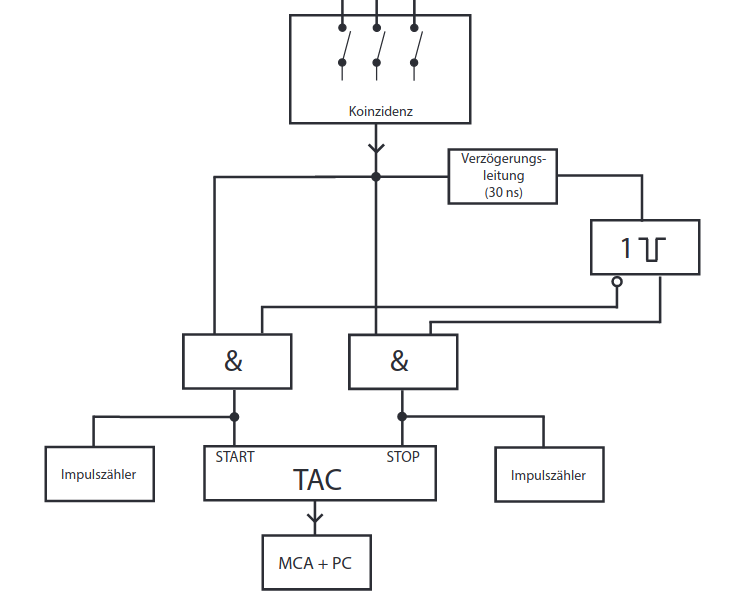
\includegraphics[width=7cm]{bilder/unten_schaltung.png}
    \caption{Der untere Teil der Schaltung aus \autoref{fig:schaltung}, zur genaueren Betrachtung \cite{anleitung}.}
    \label{fig:stoppschaltung}
\end{wrapfigure}
Im Normalzustand liegt von dem Monoflop ein HIGH an dem ersten AND-Gatter und ein LOW am zweiten AND-Gatter (links). Wird von der Koinzidenzschaltung ein Signal gegeben, so liegen am 
ersten AND-Gatter zwei HIGH Signale an, sodass ein Signal weitergegeben wird. Es wird ein Impuls gezählt und der Time-Amplitude-Converter (TAC) wird ausgelöst und startet die Zeitnahme. 
Da am zweiten AND zu dem Zeitpunkt vom Monoflop ein LOW anliegt, passiert dort nichts. Durch die Verzögerungsleitung wird der Monoflop erst $\SI{30}{\nano\second}$ später getriggert. 
Innerhalb der Suchzeit $T_\text{s}$ liegt durch den Monoflop ein LOW am ersten AND-Gatter und ein HIGH am zweiten AND-Gatter.
Läuft nun die Suchzeit ab, ohne das ein weiteres Teilchen registriert wird, geht der Monoflop in seinen Ausgangszustand zurück, der TAC verwirft die angefangene Zeitnahme. Es wird kein 
Signal weitergegeben. \\
Wird während der Suchzeit ein weiteres Signal von der Koinzidenzschaltung in die restliche Schaltung gegeben, so liegen zwei HIGH Signale am zweiten AND-Gatter, hier wird der Impuls 
gezählt und die Zeitnehmung wird am TAC gestoppt. Der Monoflop wird in seinen Ausgangszustand getriggert. \\
Am TAC wird die gemessene Zeit in einen zur ihr proportionalen Spannungspuls konvertiert. Dieser geht weiter an den Multichannelanalyser (MCA) (dt. Vielkanalanalysator). Der MCA sortiert die Spannungspulse 
nach ihrer Größe und sammelt Pulse ähnlicher Höhe in den einzelnen Kanälen. Am Computer wird ein Histogramm erzeugt, wie viele Spannungspulse in welchem Kanal gesammelt werden.\\
An der Koinzidenzschaltung ist neben den PMT noch ein Doppelpulsgenerator angeschlossen, mit dem der untere Teil der Schaltung getestet werden kann und durch welchen die Kanäle 
des MCA mit einer Zeit assoziiert werden können. 

\section{Durchführung}
\label{sec:Durchführung}

\noindent Die im Aufbau \ref{sec:Aufbau} beschriebene Schaltung wird Schritt für Schritt aufgebaut und währenddessen eingestellt. Anschließend wird die Messung von Individuallebensdauern gestartet
und mehrere Tagen laufen gelassen. \\

    \subsection{Justage}

    \noindent Die PMT werden an eine Hochspannung angeschlossen. Mit einem Oszilloskop wird sich vergewissert, dass Spannungsimpulse verschiedener Höhe sichtbar sind. 
    Die PMT werden jeweils an eine verstellbare Verzögerungsleitung angeschlossen, welche zunächst auf einer Verzögerung von $\SI{0}{\nano\second}$ stehen. Es wird ein PMT über die Verzögerungsleitung 
    mit einem Diskrimator verbunden, dann werden mit Hilfe eines Zählwerkes die Impulse pro Sekunde ermittelt. Es werden in einem Zeitraum von $\SI{10}{\nano\second}$ die ankommenden Impulse 
    gezählt. Die Schwellspannung des Diskriminators wird so eingestellt, dass in etwa $\SI{30}{\second\tothe{-1}}$ gemessen werden. Dann wird die Pulsdauer des Diskriminators auf einem 
    Oszilloskop betrachtet und so eingestellt, dass sie eine Pulsdauer von $\increment t = \SI{10}{\nano\second}$ hat. Das gleiche Vorgehen wird mit dem anderen PMT und dem anderen 
    Diskriminator wiederholt. 

        \subsubsection{Bestimmung der Verzögerungszeit}

            \noindent Damit die Koinzidenzschaltung bestmöglichst eingestellt ist, werden die Impulse der Schaltung für verschiedene Verzögerungszeiten gemessen. Dafür wird die Koinzidenzschaltung 
            an einen Impulszähler geschlossen. Die zuvor eingestellten Diskriminatoren werden inklusive der Verzögerungsleitungen und den PMTs als Input in die Koinzidenzschaltung gesteckt. 
            Nun wird für verschiedene Verzögerungszeiten die Anzahl an Impulsen in einem Intervall von $t = \SI{20}{\second}$ notiert. Dazu wird erst eine Leitung verlängert, während die andere auf 
            einer Verzögerung von $\SI{0}{\nano\second}$ steht. Danach wird die zuerst ausgemessene Leitung auf keine Verzögerung gestellt und die andere schrittweise erhöht. \\ 
            Anschließend wird eine geeignete Verzögerungszeit ausgewählt und für den weiteren Versuchsablauf eingestellt. Ein Richtwert für die Ereignisrate ist etwa $\SI{20}{\second\tothe{-1}}$.
            
    \noindent Nur wird die restliche Schaltung aufgebaut. An dem Monoflop wird eine Suchzeit von $\SI{10}{\micro\second}$ eingestellt. Der Messbereich des TAC wird dementsprechend angepasst, 
    sodass diese die Spannungspulse so bildet, dass möglichst viele Kanäle im MCA benutzt werden können. Dann stehen die verschiedenen Kanäle für feinere Zeitintervalle. 

        \subsubsection{Kalibrationsmessung}

            \noindent Die gemessenen Zeiten zwischen zwei detektierten Ereignissen wird je länge in verschiedene Kanäle im MCA sortiert und am Computer wird die Anzahl an Zeiten pro 
            Kanal abgelesen. Damit mit den Kanälen eine Zerfallszeit assoziiert werden kann, werden die PMT von der Koinzidenzschaltung gesteckt und ein Doppelpulsgenerator mit 
            einstellbarer Zeit $t_\text{a}$ zwischen den Pulsen angeschlossen. \\ 
            Es wird eine Zeit $t_\text{a}$ eingestellt, für $\SI{15}{\second}$ gemessen und anschließend der Kanal und die Anzahl der Ereignisse notiert. Es wird in Schritten von 
            $\increment t_\text{a} = \SI{0.3}{\micro\second}$ der Messbereich von $\SI{0.3}{\micro\second}$ - $\SI{9.9}{\micro\second}$ ausgemessen. 
            

    \subsection{Messung der Lebensdauer}

    \noindent Es werden die Photomultiplier wieder an die Koinzidenzschaltung angeschlossen, der Doppelpulsgenerator wird entfernt. Die Impulszähler und die Messung am Computer 
    werden zeitgleich gestartet. Die Messung sollte $\SI{20}{\hour}$ - $\SI{30}{\hour}$ laufen, damit einige Zerfallszeiten aufgenommen werden. 